\section{Geometría analítica}

%---------------------------------------------------------------------slide----
\mode<presentation>{
	\begin{frame}
		\frametitle{Geometría analítica}
		\setlength{\parskip}{0.3em}
		\tableofcontents[sectionstyle=show/hide,hideothersubsections]
	\end{frame}
}

\subsection{Vectores}

%---------------------------------------------------------------------slide----
\begin{frame}
	\frametitle{Escalares}
	Algunos fenómenos de la naturaleza pueden describirse mediante un número referido a una unidad de medida. 
	
	\begin{definicion}[Escalar]
		Un \emph{escalar} es un número que sirve para expresar una magnitud sin dirección.
	\end{definicion}
	\structure{\bfseries Ejemplos} La estatura o el peso de una persona, la temperatura de un gas o el tiempo que tarda un móvil en recorrer una distancia.
	
	Sin embargo, existen otros fenómenos que no pueden describirse adecuadamente mediante un escalar. 
	Si, por ejemplo, un navegante quiere poner rumbo a puerto y sólo conoce de la intensidad del viento, no sabrá qué dirección tomar. 
	La descripción del viento requiere dos elementos, su intensidad y su dirección. 
	
\end{frame}


%---------------------------------------------------------------------slide----
\begin{frame}
	\frametitle{Vectores}
	\begin{definicion}[Vector]
		Un \emph{vector} es un número que sirve para expresar una magnitud y tiene asociada una dirección y un sentido. 
	\end{definicion}
	
	\structure{\bfseries Ejemplos} La velocidad de un móvil o la fuerza que se aplica sobre un objeto.  
	 
	Geométricamente, un vector se representa mediante un segmento orientado, es decir, una flecha.  
	\begin{center}
		\scalebox{0.8}{\begin{pspicture}(0,-2)(11,2)
\rput(2.74,0.37890625){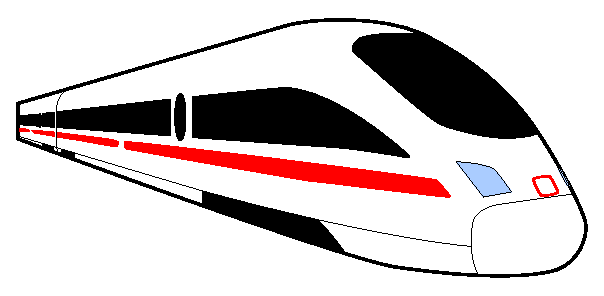
\includegraphics[scale=0.5]{img/geometria_analitica/tren.eps}}
\psline[linewidth=0.08cm,arrowsize=0.05291667cm 2.0,arrowlength=1.4,arrowinset=0.4]{->}(5.72,-0.6610938)(9.34,-1.2610937)
\usefont{T1}{ptm}{m}{n}
\rput(7.5514064,-0.69609374){$\vec{v}$}
\usefont{T1}{ptm}{m}{n}
\rput(10.043282,-1.2360938){dirección}
\psline[linewidth=0.04cm,linecolor=red,tbarsize=0.07055555cm 5.0]{|-|}(5.64,-0.9010937)(9.26,-1.5010937)
\usefont{T1}{ptm}{m}{n}
\rput(7.118906,-1.4560938){magnitud}
\end{pspicture} }
	\end{center}
\end{frame}


% ---------------------------------------------------------------------slide----
\begin{frame}
	\frametitle{Representación de un vector}
	Un segmento orientado puede ubicarse en diferentes lugares dentro de un espacio cartesiano. 
	Sin embargo, con independencia de donde esté situado, si la longitud y la dirección no varían, dicho segmento
	representará siempre el mismo vector.
	
	Esto permite representar todos los vectores con un mismo origen, el origen en sistema de coordenadas cartesianas.
	Así, un vector queda determinado por las \emph{coordenadas} de su extremo final en cualquier espacio euclideo.
	
	\begin{center}
		\scalebox{0.8}{\psset{unit=1,algebraic}
\begin{pspicture}(-4,-2.5)(4,2.5)
\psaxes[ticks=none,labels=none]{<->}(0,0)(-4,-2.5)(4,2.5)
\psline{->}(2,1.5)(4,2.5)
\rput(1.8,1.4){$A$}
\rput(4.2,2.6){$B$}
\psline{->}(-3,0.5)(-1,1.5)
\rput(-3.2,0.4){$C$}
\rput(-0.8,1.6){$D$}
\psline{->}(-1,-2)(1,-1)
\rput(-1.2,-2.1){$E$}
\rput(1.2,-0.9){$F$}
\psline[linecolor=red]{->}(0,0)(2,1)
\rput(1,0.6){$\mathbf{v}$}
\psline[linestyle=dashed, linecolor=gray](2,0)(2,1)(0,1)
\psxTick[ticksize=-3pt 0,labelsep=3pt](2){x}
\psyTick[ticksize=-3pt 0,labelsep=3pt](1){y}
\rput[l](3,0.5){${\mathbf{v}} = (x,y) = \vec{AB}=\vec{CD}=\vec{EF}$}
\end{pspicture}}
	\end{center}
\end{frame} 


% ---------------------------------------------------------------------slide----
\begin{frame}
	\frametitle{Vector a partir de dos puntos}
	Dados dos puntos $P$ y $Q$ de un espacio cartesiano, el vector con origen en $P$ y destino en $Q$ tiene coordenadas $\vec{PQ}=Q-P$.
	
	\structure{\bfseries Ejemplo} 
	Sean los puntos $P=(2,1)$  y $Q=(3,4)$ del plano real $\mathbb{R}^2$, entonces
	\[
		\vec{PQ} = Q-P = (3,4)-(2,1) = (3-2,4-1) = (1,3).
	\]
	\begin{center}
		\scalebox{0.8}{\psset{unit=1,algebraic}
\begin{pspicture}(-0.5,-0.5)(5,5)
\psaxes[labelFontSize=\scriptstyle,ticksize=-3pt 0,labelsep=2pt]{<->}(0,0)(-0.5,-0.5)(5,5)[$x$,-90][$y$,180]
\psdot(3,4)
\psline[linestyle=dashed, linecolor=gray](3,0)(3,4)(0,4)
\rput[l](3.1,4){$Q$}
\psdot(2,1)
\psline[linestyle=dashed, linecolor=gray](2,0)(2,1)(0,1)
\rput[l](2.1,1){$P$}
\psline[linecolor=red]{->}(2,1)(3,4)
\rput[r](2.4,2.5){$\vec{PQ}$}
\end{pspicture}}
	\end{center}
\end{frame} 


% ---------------------------------------------------------------------slide----
\begin{frame}
	\frametitle{Módulo de un vector}
	\begin{definicion}[Módulo de un vector]
		Dado un vector $\mathbf{v}=(v_1,\cdots,v_n)$ de $\mathbb{R}^n$, se define el \emph{módulo} de $\mathbf{v}$ como
		\[
			|\mathbf{v}| = \sqrt{v_1^2+ \cdots + v_n^2}.
		\]
	\end{definicion}
	El módulo de un vector coincide con la longitud del segmento que representa al vector.
	
	\structure{\bfseries Ejemplos} 
	Sea $\mathbf{u}=(3,4)$ un vector en $\mathbb{R}^2$, entonces
	\[
		|\mathbf{u}| = \sqrt{3^2+4^2} = \sqrt{25} = 5
	\]
	Sea $\mathbf{v}=(4,7,4)$ un vector en $\mathbb{R}^3$, entonces
	\[
		|\mathbf{v}| = \sqrt{4^2+7^2+4^2} = \sqrt{81} = 9
	\]
\end{frame} 


% ---------------------------------------------------------------------slide----
\begin{frame}
	\frametitle{Vectores unitarios}
	\begin{definicion}[Vector unitario]
		Se dice que un vector $\mathbf{v}$ de $\mathbb{R}^n$ es \emph{unitario} si su módulo es 1, es decir $|\mathbf{v}|=1$.
	\end{definicion}
	Especial atención merecen los vectores unitarios que siguen la dirección de los ejes de coordenadas, estos vectores se llaman \emph{vectores coordenados}.
	\begin{columns}
		\begin{column}{.48\textwidth}
			En $\mathbb{R}^2$ los vectores coordenados son 
			\[
				\mathbf{i}=(1,0)\mbox{ y }\mathbf{j}=(0,1)
			\]
			\begin{center}
				\scalebox{1}{\psset{unit=1,algebraic}
\begin{pspicture}(-0.5,-0.5)(2.5,2.5)
\psaxes[labelFontSize=\scriptstyle,ticksize=-3pt 0,labelsep=2pt]{<->}(0,0)(-0.5,-0.5)(2,2)[$x$,-90][$y$,180]
\psline[linecolor=red]{->}(0,0)(1,0)
\rput(0.5,0.2){$\mathbf{i}$}
\psline[linecolor=red]{->}(0,0)(0,1)
\rput(0.2,0.5){$\mathbf{j}$}
\end{pspicture}}
			\end{center}
		\end{column}
		\begin{column}{.48\textwidth}
			En $\mathbb{R}^3$ los vectores coordenados son 
			\[
				\mathbf{i}=(1,0,0)\mbox{, }\mathbf{j}=(0,1,0) \mbox{ y } \mathbf{k}=(0,0,1)
			\]
			\begin{center}
				\scalebox{1}{\psset{unit=1}
\psset{viewpoint=40 20 20 , Decran=50}
\begin{pspicture}(-0.5,-0.5)(2,2)
\axesIIID(0,0,0)(2,2,2)
\psPoint(0,0,0){O}
\psPoint(1,0,0){i}
\psPoint(0,1,0){j}
\psPoint(0,0,1){k}
\psline[linecolor=red]{->}(O)(i)
\uput[r](i){$\mathbf{i}$}
\psline[linecolor=red]{->}(O)(j)
\uput[u](j){$\mathbf{j}$}
\psline[linecolor=red]{->}(O)(k)
\uput[r](k){$\mathbf{k}$}
\end{pspicture}}
			\end{center}
		\end{column}   
	\end{columns}
\end{frame} 


% ---------------------------------------------------------------------slide----
\begin{frame}
	\frametitle{Suma de vectores}
	\begin{definicion}[Suma de vectores]
		Dados dos vectores $\mathbf{u}=(u_1,\cdots,u_n)$ y $\mathbf{v}=(v_1,\cdots,v_n)$ de $\mathbb{R}^n$, se define la
		\emph{suma} de $\mathbf{u}$ y $\mathbf{v}$ como
		\[
			\mathbf{u}+\mathbf{v} = (u_1+v_1,\ldots, u_n+v_n).
		\]
	\end{definicion}
	
	\structure{\bfseries Ejemplo} 
	Sean $\mathbf{u}=(3,1)$ y $\mathbf{v}=(2,3)$ dos vectores en $\mathbb{R}^2$, entonces
	\[
		\mathbf{u}+\mathbf{v} = (3+2,1+3) = (5,4).
	\]
	
	\begin{center}
		\scalebox{0.8}{\psset{unit=1,algebraic}
\begin{pspicture}(-0.5,-0.5)(5,4)
\psaxes[ticks=none,labels=none]{<->}(0,0)(-0.5,-0.5)(5,4)[$x$,-90][$y$,180]
\psline{->}(0,0)(3,1)
\rput(1.6,0.3){$\mathbf{u}$}
\psline[linestyle=dashed, linecolor=gray](3,0)(3,1)(0,1)
\psxTick[ticksize=-3pt 0,labelsep=3pt](3){u_1}
\psyTick[ticksize=-3pt 0,labelsep=3pt](1){u_2}
\psline{->}(0,0)(1,2)
\rput(0.4,1.2){$\mathbf{v}$}
\psline[linestyle=dashed, linecolor=gray](1,0)(1,2)(0,2)
\psxTick[ticksize=-3pt 0,labelsep=3pt](1){v_1}
\psyTick[ticksize=-3pt 0,labelsep=3pt](2){v_2}
\psline[linecolor=red]{->}(0,0)(4,3)
\rput(2,1.6){$\mathbf{u}+\mathbf{v}$}
\psline[linestyle=dashed, linecolor=gray](4,0)(4,3)(0,3)
\psxTick[ticksize=-3pt 0,labelsep=3pt](4){u_1+v_1}
\psyTick[ticksize=-3pt 0,labelsep=3pt](3){u_2+v_2}
\psline[linestyle=dashed, linecolor=gray](3,1)(4,3)
\psline[linestyle=dashed, linecolor=gray](1,2)(4,3)
\end{pspicture}}
	\end{center}
\end{frame} 


%---------------------------------------------------------------------slide----
\begin{frame}
	\frametitle{Producto de un vector por un escalar}
	\begin{definicion}[Producto de un vector por un escalar]
		Dado un vector $\mathbf{v}=(v_1,\cdots,v_n)$ de $\mathbb{R}^n$, y un escalar $a\in \mathbb{R}$, se define el
		\emph{producto} de $a$ por $\mathbf{v}$ como
		\[
			a\mathbf{v} = (av_1,\ldots, av_n).
		\]
	\end{definicion}
	\structure{\bfseries Ejemplo}
	Sean el vector $\mathbf{v}=(2,1)$ en $\mathbb{R}^2$ y el escalar $a=2$, entonces
	\[
		a\mathbf{v} = 2(2,1) = (4,2).
	\]
	
	\begin{center}
		\scalebox{0.8}{\psset{unit=1,algebraic}
\begin{pspicture}(-0.5,-0.5)(5,3)
\psaxes[ticks=none,labels=none]{<->}(0,0)(-0.5,-0.5)(5,3)[$x$,-90][$y$,180]
\psline[linecolor=red]{->}(0,0)(4,2)
\rput(2.2,1.3){$a\mathbf{v}$}
\psline[linestyle=dashed, linecolor=gray](4,0)(4,2)(0,2)
\psxTick[ticksize=-3pt 0,labelsep=3pt](4){av_1}
\psyTick[ticksize=-3pt 0,labelsep=3pt](2){av_2}
\psline{->}(0,0)(2,1)
\rput(0.9,0.7){$\mathbf{v}$}
\psline[linestyle=dashed, linecolor=gray](2,0)(2,1)(0,1)
\psxTick[ticksize=-3pt 0,labelsep=3pt](2){v_1}
\psyTick[ticksize=-3pt 0,labelsep=3pt](1){v_2}
\end{pspicture}}
	\end{center}
\end{frame}  


%---------------------------------------------------------------------slide----
\begin{frame}
	\frametitle{Expresión de un vector como combinación lineal de los vectores coordenados}
	La suma de vectores y el producto de un vector por un escalar permite expresar cualquier vector como una combinación lineal de los vectores coordenados.
	
	En el caso del espacio real $\mathbb{R}^3$, cualquier vector $\mathbf{v}=(v_1,v_2,v_3)$ puede expresarse como   
	\[
		\mathbf{v}=(v_1,v_2,v_3) = v_1\mathbf{i}+v_2\mathbf{j}+v_3\mathbf{k}.
	\]
	
	\begin{center}
		\scalebox{0.8}{\psset{unit=1}
\psset{viewpoint=40 20 20,Decran=50}
\begin{pspicture}(0,0)(3,3)
\axesIIID(0,0,0)(3,3,3)
\psPoint(0,0,0){O}
\psPoint(1,0,0){i}
\psPoint(0,1,0){j}
\psPoint(0,0,1){k}
\psPoint(1,2,3){v}
\psline[linecolor=red]{->}(O)(i)
\uput[r](i){$\mathbf{i}$}
\psline[linecolor=red]{->}(O)(j)
\uput[u](j){$\mathbf{j}$}
\psline[linecolor=red]{->}(O)(k)
\uput[r](k){$\mathbf{k}$}
\psline[linecolor=blue]{->}(O)(v)
\psPoint(1,1.4,2){v2}
\uput[r](v2){$\mathbf{v}$}
\psPoint(1,2,0){xy}
\psPoint(0,2,0){j2}
\psline[linestyle=dashed, linecolor=gray](i)(xy)(j2)
\psline[linestyle=dashed, linecolor=gray](xy)(v)
\psPoint(1,0,3){xz}
\psPoint(0,0,3){k3}
\psline[linestyle=dashed, linecolor=gray](i)(xz)(k3)
\psline[linestyle=dashed, linecolor=gray](xz)(v)
\psPoint(0,2,3){yz}
\psline[linestyle=dashed, linecolor=gray](j2)(yz)(k3)
\psline[linestyle=dashed, linecolor=gray](yz)(v)
\psPoint(1,1,0){a}
\uput[d](a){$v_2$}
\psPoint(0.8,2,0){b}
\uput[r](b){$v_1$}
\psPoint(0,2,1.5){c}
\uput[r](c){$v_3$}
\end{pspicture}}
	\end{center}
\end{frame} 


%---------------------------------------------------------------------slide----
\begin{frame}
	\frametitle{Producto escalar}
	\begin{definicion}[Producto escalar]
		Dados dos vectores $\mathbf{u}=(u_1,\cdots,u_n)$ y $\mathbf{v}=(v_1,\cdots,v_n)$ de $\mathbb{R}^n$, se define el
		\emph{producto escalar} de $\mathbf{u}$ y $\mathbf{v}$ como
		\[
			\mathbf{u}\cdot \mathbf{v} = u_1v_1 + \cdots + u_nv_n.
		\]
	\end{definicion}
	\structure{\bfseries Ejemplo} 
	Sean $\mathbf{u}=(3,1)$ y $\mathbf{v}=(2,3)$ dos vectores en $\mathbb{R}^2$, entonces
	\[
		\mathbf{u}\cdot\mathbf{v} = 3\cdot 2 +1\cdot 3 = 9.
	\]
	
	Se cumple que
	\[
		\mathbf{u}\cdot\mathbf{v} =  |\mathbf{u}||\mathbf{v}|\cos\alpha
	\]
	donde $\alpha$ es el ángulo que forman los vectores.
\end{frame} 


%---------------------------------------------------------------------slide----
\begin{frame}
	\frametitle{Vectores paralelos}
	\begin{definicion}[Vectores paralelos]
		Dos vectores $\mathbf{u}$ y $\mathbf{v}$ son \emph{paralelos} si existe un valor $a\in\mathbb{R}$ tal que
		\[
			\mathbf{u} = a\mathbf{v}.
		\]
	\end{definicion}
	
	\structure{\bfseries Ejemplos} 
	Los vectores $\mathbf{u}=(-4,2)$ y $\mathbf{v}=(2,-1)$ en $\mathbb{R}^2$ son paralelos, ya que
	\[
		\mathbf{v}= (-4,2) = -2(2,-1) = -2\mathbf{v}.
	\]
	
\end{frame} 


%---------------------------------------------------------------------slide----
\begin{frame}
	\frametitle{Vectores ortogonales y ortonormales}
	\begin{definicion}[Vectores ortogonales y ortonormales]
		Dos vectores $\mathbf{u}$ y $\mathbf{v}$ son \emph{ortogonales} si su producto escalar es nulo
		\[
			\mathbf{u}\cdot \mathbf{v} = 0.
		\]
		Si además el módulo de ambos vectores es la unidad $|\mathbf{u}|=|\mathbf{v}|=1$, entonces se dice que son \emph{ortonormales}.
	\end{definicion}
	
	Los vectores ortogonales son perpendiculares entre sí, es decir, forman un ángulo de $90^\circ$.
	
	\structure{\bfseries Ejemplos} 
	Los vectores $\mathbf{u}=(2,1)$ y $\mathbf{v}=(-2,4)$ en $\mathbb{R}^2$ son ortogonales, ya que
	\[
		\mathbf{u}\mathbf{v} = 2\cdot -2 +1\cdot 4 = 0,
	\]
	pero no son ortonormales ya que $|\mathbf{u}| = \sqrt{2^2+1^2} \neq 1$ y  $|\mathbf{v}| = \sqrt{-2^2+4^2} \neq 1$.
	
	Los vectores $\mathbf{i}=(1,0)$ y $\mathbf{j}=(0,1)$ en $\mathbb{R}^2$ son ortonormales, ya que
	\[
		\mathbf{i}\mathbf{j} = 1\cdot 0 +0\cdot 1 = 0, \quad |\mathbf{i}| = \sqrt{1^2+0^2} = 1,  \quad |\mathbf j| = \sqrt{0^2+1^2} = 1.
	\]
\end{frame}  



\subsection{Rectas}
%---------------------------------------------------------------------slide----
\begin{frame}
	\frametitle{Ecuación vectorial de la recta}
	\begin{definicion}[Ecuación vectorial de la recta]
		Sea $l$ una recta del espacio $\mathbb{R}^n$ y sean $P=(p_1,\ldots,p_n)$ un punto cualquiera de la recta y
		$\mathbf{v}=(v_1,\ldots,v_n)$ un vector cualquiera con la misma dirección que la recta.
		La ecuación
		\[
			l: X= P + t\mathbf{v} = (p_1,\ldots,p_n)+t(v_1,\ldots,v_n) = (p_1+tv_1,\ldots,p_n+tv_n).
		\]
		parametriza a $l$ en función de $t\in \mathbb{R}$, y se conoce como \emph{ecuación vectorial de la recta}.
	\end{definicion}
	\begin{columns}
		\begin{column}{.48\textwidth}
			\structure{\bfseries Ejemplo} 
			Considerese la recta del espacio real $\mathbb{R}^3$ que aparece en la gráfica. Un punto de la recta es $P=(1,1,2)$ y un vector director es $\mathbf{v}=(-1,2,2)$, luego su ecuación vectorial es
			\begin{align*}
				l & : X= P + t\mathbf{v} = (1,1,2)+t(-1,2,1) = \\
				  & = (1-t,1+2t,2+t)\quad t\in\mathbb{R}.      
			\end{align*}
		\end{column}
		\begin{column}{.48\textwidth}
			\begin{center}
				\scalebox{0.8}{\psset{unit=1}
\psset{viewpoint=40 20 20,Decran=40}
\begin{pspicture}(0,0)(2,2)
\axesIIID(0,0,0)(3,3,3)
\psPoint(0,0,0){O}
\psPoint(1,1,2){P}
\psPoint(0,3,3){v}
\psSolid[object=line,args=2 -1 1 -1 5 4]
\psSolid[object=point,args=1 1 2]
\psline[linecolor=red]{->}(P)(v)
\uput[d](P){$P$}
\psPoint(0.5,2,2.5){v2}
\uput[u](v2){$\mathbf{v}$}
\psPoint(-1,5,4){l}
\uput[r](l){$l$}
\end{pspicture}}
			\end{center}
		\end{column}
	\end{columns}
\end{frame} 


%---------------------------------------------------------------------slide----
\begin{frame}
	\frametitle{Ecuaciones paramétricas y cartesianas de la recta}
	De la ecuación vectorial de una recta $l: X=P + t\mathbf{v}=(p_1+tv_1,\ldots,p_n+tv_n)$ se obtienen facilmente las coordenadas de los puntos que forman parte de la recta mediante $n$ ecuaciones paramétricas:
	\[
		x_1(t)=p_1+tv_1, \ldots, x_n(t)=p_n+tv_n
	\]
	donde, si $\mathbf{v}$ es un vector cuyas coordenadas son no nulas ($v_i\neq 0$ $\forall i$), se puede despejar el parámetro $t$ en cada una de ellas e igualarlas,
	\[
		\frac{x_1-p_1}{v_1}=\cdots = \frac{x_n-p_n}{v_n}
	\] 
	
	\structure{\bfseries Ejemplo} 
	Dada la ecuación vectorial de la recta $l: X=(1,1,2)+t(-1,2,1) =(1-t,1+2t,2+t)$ en el espacio real $\mathbb{R^3}$, sus
	ecuaciones paramétricas son
	\[
		x(t) = 1-t, \quad y(t)=1+2t, \quad z(t)=2+t,
	\]
	y sus ecuaciones cartesianas son
	\[
		\frac{x-1}{-1}=\frac{y-1}{2}=\frac{z-2}{1}
	\]
\end{frame} 


%---------------------------------------------------------------------slide----
\begin{frame}
	\frametitle{Ecuación punto-pendiente de una recta en el plano}
	En el caso particular del plano cartesiano $\mathbb{R^2}$, si se tiene una recta con ecuación vectorial $l: X=P+t\mathbf{v}=(x_0,y_0)+t(a,b)
	= (x_0+ta,y_0+tb)$, sus ecuaciones paramétricas son
	\[
		x(t)=x_0+ta,\quad y(t)=y_0+tb
	\]
	y sus ecuación cartesiana es
	\[
		\frac{x-x_0}{a} = \frac{y-y_0}{b}.
	\]  
	A partir de aquí, pasando $b$ multiplicando al otro lado de la ecuación, se obtiene 
	\[
		y-y_0 = \frac{b}{a}(x-x_0) \mbox{ o bien } y-y_0+m(x-x_0),
	\]
	llamando $m=b/a$. Esta ecuación se conoce como ecuación en la forma \emph{punto-pendiente}.
	 
\end{frame} 


%---------------------------------------------------------------------slide----
\begin{frame}
	\frametitle{Pendiente de una recta en el plano}
	\begin{definicion}[Pendiente de una recta]
		Dada una recta $l: X=P+t\mathbf{v}$ en el plano real $\mathbb{R}^2$, con vector director $\mathbf{v}=(a,b)$, se define la pendiente de $l$ como $b/a$.
	\end{definicion}
	
	Recordar que dados dos puntos $Q=(x_1,y_1)$ y $Q=(x_2,y_2)$ de la recta $l$, se puede tomar como vector director el vector que los une, que tiene coordenadas $\vec{PQ}=Q-P=(x_2-x_1,y_2-y_1)$, de manera que la pendiente de $l$ será 
	$\dfrac{y_2-y_1}{x_2-x_1}$, es decir, el cociente entre lo que cambia la coordenada $y$ y lo que cambia la coordenada $x$.
	
	\begin{center}
		\scalebox{0.7}{\psset{unit=1,algebraic}
\begin{pspicture*}(-0.5,-0.5)(5.2,4.2)
\psaxes[ticks=none,labels=none]{<->}(0,0)(-0.5,-0.5)(5,4)[$x$,-90][$y$,180]
\psdot(4,3)
\psline[linestyle=dashed, linecolor=gray](4,0)(4,3)(0,3)
\rput[l](4.1,2.9){$Q$}
\psdot(1,1)
\psline[linestyle=dashed, linecolor=gray](1,0)(1,1)(0,1)
\rput[u](1,1.2){$P$}
\psline(-2,-1)(7,5)
\psline[linecolor=red]{->}(1,1)(4,3)
\rput[r](2.5,2.5){$\vec{PQ}$}
\psline[linestyle=dashed, linecolor=orange](1,1)(4,1)(4,3)
\psxTick[ticksize=-3pt 0,labelsep=3pt](1){x_1}
\psxTick[ticksize=-3pt 0,labelsep=3pt](4){x_2}
\psyTick[ticksize=-3pt 0,labelsep=3pt](1){y_1}
\psyTick[ticksize=-3pt 0,labelsep=3pt](3){y_2}
\rput[u](2.5,0.8){$x_2-x_1$}
\rput[l](4.1,2){$y_2-y_1$}
\rput[l](4.1,2){$y_2-y_1$}
\rput[l](4.7,3.7){$l$}
\end{pspicture*}}
	\end{center}
\end{frame} 



\subsection{Planos}
%---------------------------------------------------------------------slide----
\begin{frame}
	\frametitle{Ecuación del plano en el espacio real}
	Para llegar a la ecuación de un plano en el espacio real $\mathbb{R}^3$ se puede partir de un punto del plano $P=(x_0,y_0,z_0)$ y de un vector perpendicular al plano $\mathbf{v}=(a,b,c)$. 
	Entonces, para cualquier punto del plano $Q=(x,y,z)$ se cumple que el vector $\vec{PQ} = (x-x_0,y-y_0,z-z_0)$ es ortogonal a $\mathbf{v}$, por lo que su producto escalar se anulará
	\[
		\vec{PQ}\cdot\mathbf{v} = (x-x_0,y-y_0,z-z_0)(a,b,c) = a(x-x_0)+b(y-y_0)+c(z-z_0) = 0.
	\]
	
	\begin{center}
		\scalebox{0.8}{\psset{unit=1,viewpoint=40 10 5,Decran=40}
\begin{pspicture}(-3,-3)(5,4)
\psSolid[object=plan, definition=normalpoint, args={1 1 1 [1 2 2]}, fillcolor=cyan, base=-2 2 -2 2]
\psSolid[object=point,args=1 1 1]
\psPoint(1,1,1){P}
\uput[l](P){$P$}
\psPoint(1,2,0){Q}
\uput[d](Q){$Q$}
\psline{->}(P)(Q)
\psPoint(1,2,2){v}
\uput[r](v){$\mathbf{v}$}
\psline[linecolor=red]{->}(P)(v)
\axesIIID(0,0,0)(5,4,3.5)
\end{pspicture}}
	\end{center}
\end{frame} 



